\chapter{Systementwurf}
\label{chapter:SystemDesign}

\section{Systemzerlegung}
Bei der Systemzerlegung wird das System, basierend auf dem Anwendungsfall- und dem Analysemodell, in kleinere
Bestandteile zerlegt\cite[S. 257ff]{Bruegge_2004}.\\

Das System von Cydonia wurde in folgende Pakete zerlegt: Player, Equipment, GameWorld, GameController, Input.
Die Pakete Player und Equipment enthalten jeweils die zur Abbildung und Berechnung der Spieler bzw. der verschiedenen
Equipments ben�tigten Klassen.\\

Das Paket GameWorld fasst alle Klassen zusammen, die f�r die Generierung, Komposition, Simulation und Darstellung der
Spielwelt verantwortlich sind. Dazu geh�ren die Entit�ten f�r die Weltobjekte (Cube, Flagge, Spawnpunkt) sowie
Kontrollklassen, Fabriken und Schnittstellen.\\

Das Paket Input enth�lt die Klassen zur Verarbeitung von Benutzereingaben. Unter anderem werden darin variable
Tastenbelegungen und die Erzeugung von Steuerbefehlen implementiert.\\

Im Paket GameController befinden sich schlie�lich alle Klassen, die zur Initialisierung des Systems, Verwaltung von
Programmzust�nden und Steuerung von Men�s ben�tigt werden. Au�erdem wird hier auch die Logik, also der eigentliche
Ablauf, des Spiels umgesetzt.\\

Eine �bersicht �ber die Paketstruktur von Cydonia gibt auch Abbildung \ref{figure:global_control_flow}.

\begin{figure}[htbp]
\centering
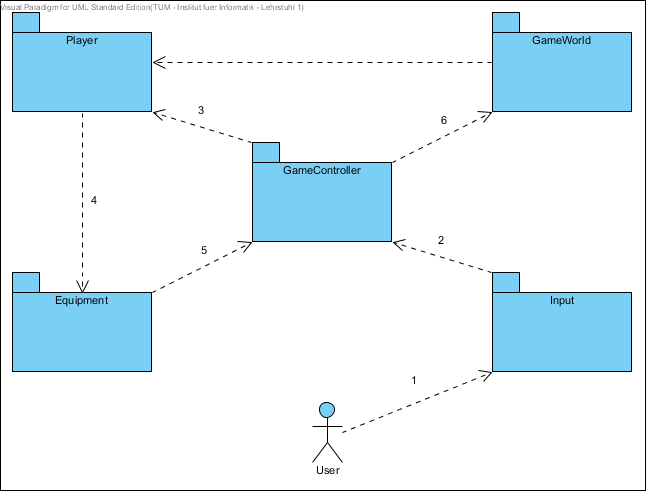
\includegraphics[width=1.0\textwidth]{images/global_control_flow}
\caption[UML-Paketdiagramm: Globaler Kontrollfluss]{UML-Paketdiagramm: Globaler Kontrollfluss}
\label{figure:global_control_flow}
\end{figure}

\section{Globaler Kontrollfluss}
\label{section:GlobalControlFlow}
Der f�r Computerspiele typische Kontrollfluss geht vom Spieler aus, der mit seinen Eingaben Ereignisse ausl�st.
Beispielsweise k�nnte der Spieler eine Taste dr�cken mit dem Ziel, einen Cube (mithilfe des Pick'n'Place-Equipments) in
der Spielwelt zu platzieren. Der Tastendruck wird vom Paket Input detektiert und in einen Steuerbefehl umgesetzt (z.B.
"`benutze equipment"'), welcher dann an das GameController-Paket weitergereicht wird. Dieses ermittelt die daraus
resultierende Reaktion, n�mlich dem Player-Paket den Befehl zu geben, das aktuelle Equipment des Spielers zu ermitteln
und dessen Benutzung anzusto�en, wodurch der Befehl im Equipment-Paket landet. Dort ist die auszuf�hrende Aktion f�r das
Pick'n'Place-Equipment implementiert (R�ckmeldungen f�r den Spieler, Manipulation der Spielwelt usw.).
Das Equipment-Paket meldet folglich dem GameController-Paket die gew�nschte Manipulation der Spielwelt, n�mlich das
Platzieren des im Equipment vorr�tigen Cubes an einer bestimmten Position. Letzendlich wird die Platzierung des Cubes im
Paket GameWorld ausgef�hrt und der Spieler kann den neuen Cube sehen. Dieser beispielhafte Ablauf kann auch anhand der
Nummerierung in Abbildung \ref{figure:global_control_flow} nachvollzogen werden.\\

Das Spiel hat jedoch auch Komponenten, die nicht ereignisgesteuert arbeiten. Das Rendern der virtuellen Welt sowie
deren physikalische Simulation laufen prozedural ab. In einer endlosen Schleife wird mehrmals pro Sekunde ein kleiner
Schritt des physikalischen Modells berechnet und ein neues Bild erzeugt.

\section{Hardware-Software Mapping}
Cydonia ist als Multiplayer-Spiel so konzipiert, dass mehrere Spieler zusammen in einer virtuellen Umgebung spielen.
Dabei nutzt jeder Spieler seinen eigenen Personal Computer (PC) (wie bei einem Singleplayer-Spiel) und die virtuelle
Welt wird zwischen den einzelnen Computern synchronisiert, damit alle Spieler den Lauf der Dinge konsistent erleben.
Dazu ist ein sog. Server n�tig, eine Instanz des Spiels, die die Autorit�t �ber die Geschehnisse in der virtuellen Welt
besitzt, da sonst durch geringf�gige Abweichungen in der Berechnung enorme Unterschiede zwischen den Simulationen auf
den einzelnen Computern entstehen k�nnen. Dieser Server kann bei ausreichender Rechenleistung auch auf einem der PCs der
Spieler laufen, der Einfachkeit halber soll im Folgenden jedoch nur der Fall eines dedizierten Servers betrachtet
werden. Abbildung \ref{figure:hardware_mapping} veranschaulicht die Verteilung der Software-Komponenten auf die
Hardware-Knoten.

\begin{figure}[htbp]
\centering
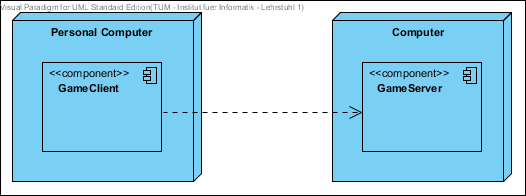
\includegraphics[width=0.8\textwidth]{images/hardware_mapping}
\caption[UML-Verteilungsdiagramm: Beziehung zwischen Software-Komponenten und Hardware-Knoten]{UML-Verteilungsdiagramm: Beziehung zwischen Software-Komponenten und Hardware-Knoten}
\label{figure:hardware_mapping}
\end{figure}
